\documentclass[11pt,a4paper]{article}

% ---- Packages ----
\usepackage[utf8]{inputenc}
\usepackage[T1]{fontenc}
\usepackage[english]{babel}
\usepackage[margin=1.1in]{geometry}
\usepackage{amsmath, amssymb, amsthm, mathtools}
\usepackage{bm}
\usepackage{booktabs, array}
\usepackage{enumitem}
\usepackage{xcolor}
\usepackage{graphicx}
\usepackage{epigraph}
\usepackage{csquotes}
\usepackage{tikz}
\usetikzlibrary{arrows.meta, positioning, shapes.geometric, shapes.misc,
                fit, calc, backgrounds, decorations.pathreplacing,
                patterns, matrix}
\usepackage{pgfplots}
\pgfplotsset{compat=1.18}
\usepackage{listings}
\usepackage[colorlinks=true, linkcolor=black!70!blue,
            citecolor=black!70!blue, urlcolor=black!40!blue]{hyperref}

% ---- Theorem environments ----
\theoremstyle{definition}
\newtheorem{definition}{Definition}[section]
\newtheorem{example}[definition]{Example}
\newtheorem{exercise}[definition]{Exercise}

\theoremstyle{remark}
\newtheorem{remark}[definition]{Remark}
\newtheorem*{aside}{Aside}

\theoremstyle{plain}
\newtheorem{proposition}[definition]{Proposition}
\newtheorem{observation}[definition]{Observation}

% ---- Epigraph style ----
\setlength{\epigraphwidth}{0.6\textwidth}
\renewcommand{\epigraphflush}{flushright}
\renewcommand{\textflush}{flushright}
\renewcommand{\epigraphsize}{\small\itshape}

% ---- Listings ----
\definecolor{codebg}{RGB}{248,248,245}
\definecolor{codekw}{RGB}{30,90,160}
\definecolor{codecm}{RGB}{110,110,110}
\lstset{
  basicstyle=\ttfamily\small,
  backgroundcolor=\color{codebg},
  keywordstyle=\color{codekw}\bfseries,
  commentstyle=\color{codecm}\itshape,
  frame=single,
  framerule=0.3pt,
  rulecolor=\color{black!30},
  breaklines=true,
  showstringspaces=false,
  language=Python,
  columns=fullflexible
}

% ---- Small conveniences ----
\newcommand{\GB}{\,\text{GB}}
\newcommand{\MB}{\,\text{MB}}
\newcommand{\TB}{\,\text{TB}}
\newcommand{\FLOPS}{\,\text{FLOPS}}
\newcommand{\TFLOPS}{\,\text{TFLOPS}}
\newcommand{\us}{\,\mu\text{s}}
\newcommand{\ms}{\,\text{ms}}

% ---- Title ----

\title{\Huge\bfseries The Arithmetic of Deep Learning\\[0.3em]
\large\mdseries\itshape Memory, Compute, Communication, and the Economics of Scale}
\author{\normalsize Lecture notes after Mikhail Khruschev (Yandex, Alice AI)\\
\small\itshape LLM Scaling Intensive}
\date{\small Transcribed and edited}

\begin{document}
\sloppy
\maketitle


\begin{abstract}
\noindent These notes accompany a lecture on the practical arithmetic that governs modern deep learning: the interplay of memory bandwidth, floating-point throughput, collective communication, and the hierarchical topology of present-day accelerators. The treatment proceeds from the lifecycle of a single training iteration to the orchestration of thousand-GPU clusters training trillion-parameter models. Throughout, the guiding principle is that one does not \emph{intuit} performance; one \emph{computes} it. Every hardware choice, every parallelism strategy, and every architectural decision is, at bottom, an exercise in back-of-the-envelope estimation --- and the envelope is what these notes attempt to sketch.
\end{abstract}

\tableofcontents
\vspace{1em}
\hrule
\vspace{1em}

% =====================================================================
\section{Prologue: The Lifecycle of an Iteration}
\label{sec:prologue}

Before examining any architecture in detail, it is instructive to consider the canonical training iteration in its most naive form. The process is deceptively simple:
\begin{enumerate}[leftmargin=1.5em,itemsep=0.2em]
    \item The CPU issues a query to the storage layer and retrieves raw data.
    \item The CPU performs preprocessing: tokenization, collation, perhaps augmentation.
    \item The assembled batch is transferred to the GPU, which computes the forward pass, the backward pass, and the optimizer step.
\end{enumerate}

Executed sequentially, this pipeline commits the cardinal sin of high-performance computing: it leaves the most expensive resource in the system --- the GPU --- waiting for the cheapest. Every millisecond of GPU idleness, multiplied by thousands of devices and millions of iterations, converts directly into wasted capital.

\begin{remark}[The dataloader imperative]
The remedy is elementary but essential: \emph{prefetching}. Data preparation must be moved to a separate, asynchronous process so that while the GPU consumes batch $n$, the CPU is already assembling batch $n+1$. This observation generalizes. The entire discipline of efficient training can be summarized as the art of overlapping expensive waits with useful work.
\end{remark}

% =====================================================================
\section{The Anatomy of a Transformer Block}
\label{sec:anatomy}

A decoder-only transformer is, structurally, a monotonous stack of identical blocks bracketed by an embedding and an unembedding. Data flows through the stack as follows:

\begin{center}
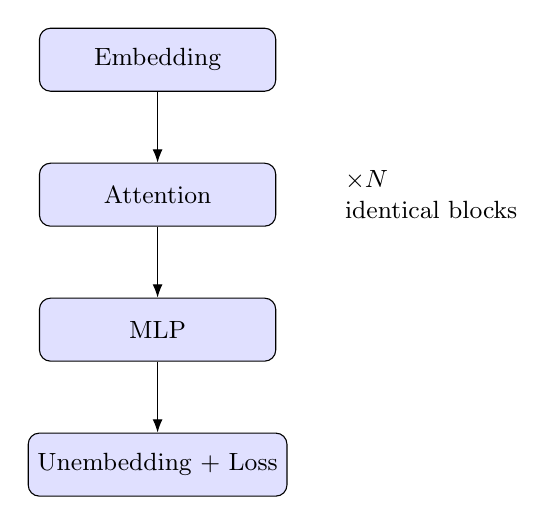
\begin{tikzpicture}[node distance=0.9cm, every node/.style={font=\small}]
  \tikzstyle{blk}=[rectangle,draw,rounded corners,fill=blue!12,minimum width=3cm,minimum height=0.8cm]
  \node[blk] (emb) {Embedding};
  \node[blk, below=of emb] (att) {Attention};
  \node[blk, below=of att] (mlp) {MLP};
  \node[blk, below=of mlp] (unemb) {Unembedding + Loss};
  \draw[-Latex] (emb) -- (att);
  \draw[-Latex] (att) -- (mlp);
  \draw[-Latex] (mlp) -- (unemb);
  \node[right=0.75cm of att, align=left, font=\small] { $\times N$\\ identical blocks};
\end{tikzpicture}
\end{center}

\subsection{Where the memory goes}

For a model with $N$ parameters trained with AdamW in mixed precision, memory consumption partitions into four components:
\begin{align}
\text{Weights (BF16)}    &\approx 2N \text{ bytes}, \\
\text{Gradients (BF16)}  &\approx 2N \text{ bytes}, \\
\text{Optimizer states (FP32, first and second moments)} &\approx 8N \text{ bytes}, \\
\text{Master weights (FP32)} &\approx 4N \text{ bytes}.
\end{align}
This gives roughly $16N$ bytes for the \emph{resident} state alone, before activations enter the picture. For a 1B parameter model, this amounts to approximately $31.5\GB$; for Llama-70B, hundreds of gigabytes; for configurations such as Qwen-235B-A32B, total training-time memory enters the \emph{terabyte} regime.

\begin{example}[Qwen 235B-A32B, per-block accounting]
Tracing activations and weight gradients through the block reveals a striking asymmetry:
\begin{center}
\begin{tabular}{lrr}
\toprule
Component & Weights/gradients & Activations \\
\midrule
Attention     & $142 \MB$        & $352 \MB$ \\
MLP           & $4{,}831 \MB$    & $1{,}000 \MB$ \\
\bottomrule
\end{tabular}
\end{center}
Aggregated, the model demands on the order of $4.8\TB$ of working memory, against an AdamW optimizer footprint of roughly $4.23\TB$. A single H100 provides $80$--$94\GB$. The disparity is not a bug but a design parameter: it \emph{forces} the use of sharding, offloading, and recomputation.
\end{example}

% =====================================================================
\section{Cartography of the GPU}
\label{sec:gpu}


Effective optimization is impossible without an accurate map of the hardware. We map in two senses: the \emph{topology} (what is connected to what) and the \emph{cost} (at what rate data can traverse each edge). Three routes lead to the map --- consulting domain experts, reading technical specifications, and performing direct measurement --- and a prudent practitioner uses all three.

\subsection{H100 SXM versus H100 NVL}

\begin{center}
\begin{tabular}{lrr}
\toprule
Metric & H100 SXM & H100 NVL \\
\midrule
TF32 Tensor Core\textsuperscript{*}    & $989\TFLOPS$   & $835\TFLOPS$ \\
BF16 Tensor Core\textsuperscript{*}    & $1{,}979\TFLOPS$ & $1{,}671\TFLOPS$ \\
FP8  Tensor Core\textsuperscript{*}    & $3{,}958\TFLOPS$ & $3{,}341\TFLOPS$ \\
GPU memory                             & $80\GB$   & $94\GB$ \\
HBM bandwidth                          & $3.35\TB/\text{s}$ & $3.9\TB/\text{s}$ \\
NVLink                                 & $900\GB/\text{s}$  & $600\GB/\text{s}$ \\
PCIe Gen5                              & $128\GB/\text{s}$  & $128\GB/\text{s}$ \\
\bottomrule
\end{tabular}
\end{center}

\begin{remark}[The asterisk]
The starred figures assume 2{:}4 structured sparsity --- at least one zero in every pair of consecutive weights. Dense workloads see roughly half these numbers. Furthermore, realized throughput typically trails the datasheet by a further factor: empirical HBM bandwidth of $2.4$--$2.8\TB/\text{s}$ is a reasonable working assumption. The specification is a ceiling; the achievable is a negotiation.
\end{remark}

\subsection{Memory hierarchy}

Within a single H100 SXM, capacity grows and latency worsens monotonically as one descends the hierarchy:

\begin{center}
\begin{tabular}{lll}
\toprule
Level & Capacity & Effective bandwidth \\
\midrule
Registers (per SM)          & $64\,\text{KB}$   & --- \\
Shared memory (per SM)      & $256\,\text{KB}$  & combined $\approx 31\TB/\text{s}$ \\
L2 cache                    & $50\,\text{MB}$   & --- \\
HBM                         & $80\GB$    & $2.4\TB/\text{s}$ (practical) \\
Host RAM                    & $0.8$--$3\TB$ & $256\GB/\text{s}$ (to CPU) \\
NIC (InfiniBand)            & ---        & $50\GB/\text{s}$ \\
SSD                         & ---        & $12\GB/\text{s}$ \\
\bottomrule
\end{tabular}
\end{center}

The H100 chip itself contains $132$ Streaming Multiprocessors (SMs), each executing threads grouped into warps over CUDA and Tensor Cores. The B200 inherits this structure and adds a dedicated Tensor Memory tier, further accelerating matrix-heavy workloads.

\subsection{The host system}

A single eight-GPU H100 SXM host is a small federation of bandwidths:

\begin{center}
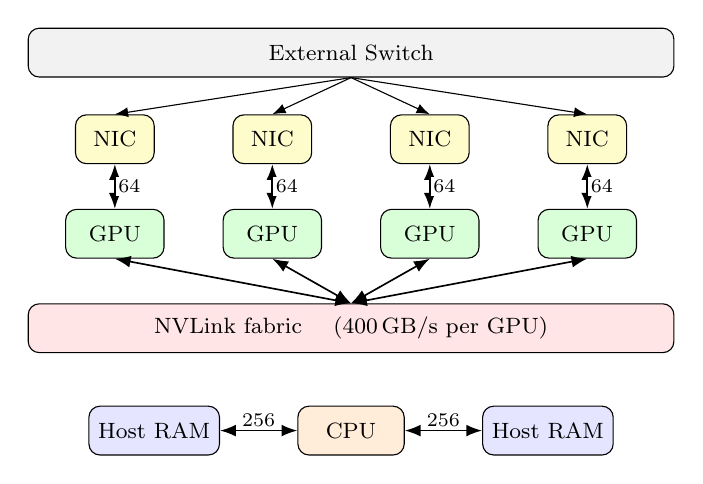
\begin{tikzpicture}[x=1cm,y=1cm,every node/.style={font=\footnotesize},
    link/.style={Latex-Latex,semithick}]
  \tikzstyle{box}=[rectangle,draw,rounded corners,minimum height=0.62cm,align=center]
  \tikzstyle{gpu}=[box,fill=green!15,minimum width=1.25cm]
  \tikzstyle{cpu}=[box,fill=orange!15,minimum width=1.35cm]
  \tikzstyle{nic}=[box,fill=yellow!20,minimum width=1.0cm]
  \tikzstyle{ram}=[box,fill=blue!10,minimum width=1.25cm]

  \node[box,minimum width=8.2cm,fill=gray!10] (sw) at (0,2.55) {External Switch};
  \foreach \x/\n in {-3.0/1,-1.0/2,1.0/3,3.0/4} {
    \node[nic] (nic\n) at (\x,1.45) {NIC};
    \node[gpu] (gpu\n) at (\x,0.25) {GPU};
    \draw[-Latex] (sw.south) -- (nic\n.north);
    \draw[link] (nic\n.south) -- node[right,font=\scriptsize,fill=white,inner sep=1pt] {64} (gpu\n.north);
  }
  \node[cpu] (cpu) at (0,-2.25) {CPU};
  \node[ram] (ram1) at (-2.5,-2.25) {Host RAM};
  \node[ram] (ram2) at (2.5,-2.25) {Host RAM};
  \draw[link] (cpu.west) -- node[above,font=\scriptsize,fill=white,inner sep=1pt] {256} (ram1.east);
  \draw[link] (cpu.east) -- node[above,font=\scriptsize,fill=white,inner sep=1pt] {256} (ram2.west);
  \node[box,minimum width=8.2cm,fill=red!10] (nv) at (0,-0.95) {NVLink fabric \quad ($400\GB/\text{s}$ per GPU)};
  \foreach \x/\n in {-3.0/1,-1.0/2,1.0/3,3.0/4} {
    \draw[link] (gpu\n.south) -- (nv.north);
  }
\end{tikzpicture}
\end{center}

The hierarchy of bandwidths (all in $\GB/\text{s}$) dictates the hierarchy of parallelism: NVLink ($\approx 400$) favors tensor parallelism; NIC ($\approx 50$) constrains data parallelism across hosts; PCIe ($\approx 64$) bottlenecks host--device transfers.

\subsection{Profiling}

The map is an abstraction; the profiler is the ground truth. Two tools dominate:
\begin{itemize}[leftmargin=1.5em,itemsep=0.2em]
    \item \texttt{torch.profiler} --- integrated with PyTorch, ideal for operator-level attribution.
    \item \texttt{nsys} (NVIDIA Nsight Systems) --- system-wide, with GPU-stream and CPU-thread timelines.
\end{itemize}
The canonical diagnostic is the \emph{GPU stream}: its density of occupancy determines utilization. Gaps betray bottlenecks --- almost always CPU-bound, communication-bound, or kernel-launch-bound. Identifying which is a prerequisite to fixing any of them.

% =====================================================================
\section{Arithmetic Intensity: A Quartet of Exercises}
\label{sec:intensity}


A computation is \emph{memory-bound} if its total data movement, divided by memory bandwidth, exceeds its total arithmetic, divided by compute throughput. This simple comparison --- the essence of the roofline model --- is the single most useful estimate in performance engineering. We now illustrate it in four settings. Throughout, we assume a single H100 with $800\TFLOPS$ of BF16 compute (a realistic, not peak, figure) and $2.4\TB/\text{s}$ of HBM bandwidth.

\subsection{Exercise 1: Elementwise addition}

\begin{exercise}
Compute $C = A + B$ for $A,B,C \in \mathbb{R}^{8192 \times 8192}$ in BF16.
\end{exercise}

The operation requires reading two matrices and writing one, at $2$ bytes per element:
\begin{equation}
T_{\text{mem}} = \frac{8192^2 \cdot 2 \cdot 3}{2.4 \cdot 10^{12}} \approx 168\us.
\end{equation}
The arithmetic is a single fused addition per element:
\begin{equation}
T_{\text{comp}} = \frac{8192^2}{800 \cdot 10^{12}} \approx 0.08\us,
\end{equation}
which, once the overhead of kernel launch ($6$--$12\us$) is included, remains utterly dominated by $T_{\text{mem}}$. The operation is, emphatically, memory-bound. Tensor Cores here are irrelevant; what matters is how many bytes the HBM can deliver per second.

\subsection{Exercise 2: Small matrix multiplication}

\begin{exercise}
Compute $C = A B$ for $A,B \in \mathbb{R}^{1024 \times 1024}$ in BF16.
\end{exercise}

Transfer:
\begin{equation}
T_{\text{mem}} = \frac{1024^2 \cdot 2 \cdot 3}{2.4 \cdot 10^{12}} \approx 2.6\us.
\end{equation}
A matrix multiplication of two $N \times N$ matrices requires $2N^3$ FMA-counted operations:
\begin{equation}
T_{\text{comp}} = \frac{2 \cdot 1024^3}{800 \cdot 10^{12}} \approx 2.6\us.
\end{equation}
The regime is balanced --- we sit on the roofline's inflection. A modest increase in $N$ tips the scale decisively: since compute grows as $N^3$ while transfer grows as $N^2$, large matmuls are compute-bound. This cubic-versus-quadratic asymmetry is the mathematical reason deep learning is viable at all.

\subsection{Exercise 3: Skinny matrix multiplication}

\begin{exercise}
Compute $C = A B$ with $A \in \mathbb{R}^{4 \times 8192}$ and $B \in \mathbb{R}^{8192 \times 8192}$.
\end{exercise}

Transfer is dominated by the large $B$:
\begin{equation}
T_{\text{mem}} = \frac{8192 \cdot 8192 \cdot 2 + 8192 \cdot 4 \cdot 2}{2.4 \cdot 10^{12}} \approx 56\us.
\end{equation}
Compute, on the other hand, is dwarfed:
\begin{equation}
T_{\text{comp}} = \frac{2 \cdot 4 \cdot 8192 \cdot 8192}{800 \cdot 10^{12}} \approx 0.6\us.
\end{equation}

\begin{observation}[The inference predicament]
This skinny matmul is the signature shape of autoregressive decoding. Its $\approx 100$-fold imbalance explains why inference is, by default, catastrophically memory-bound, and why every serious inference stack is a monument to the struggle against this fact: larger batches reuse the weight matrix across queries; continuous batching amortizes idle time; speculative decoding trades compute for memory passes; KV-cache compression squeezes the hot data. The enemy is always the same: $B$ being read again.
\end{observation}

\subsection{Exercise 4: The self-attention stack}

Take the Qwen-scale configuration: sequence length $S=8192$, hidden dimension $H=4096$, $nh=64$ heads. The three stages of attention decompose cleanly.

\paragraph{Linear projections for $Q$, $K$, $V$, and output.} Four matrices of shape $H \times H$:
\begin{equation}
T_{\text{lin}} = \frac{4 \cdot S \cdot H \cdot H \cdot 2}{800 \cdot 10^{12}} \approx 1.4\ms.
\end{equation}

\paragraph{Matrix multiplications $Q K^{\!\top}$ and attention-weights-times-$V$.}
\begin{equation}
T_{\text{matmul}} = \frac{2 \cdot H \cdot S \cdot S \cdot (2{+}1)}{800 \cdot 10^{12}} \approx 2\ms.
\end{equation}

\paragraph{Scaling and softmax, which is memory-bound.}
\begin{equation}
T_{\text{softmax}} = \frac{2 \cdot nh \cdot S \cdot S \cdot 2}{2.4 \cdot 10^{12}} \approx 7.1\ms.
\end{equation}

\begin{remark}
In the naive implementation, the element-wise softmax over a $64 \times 8192 \times 8192$ tensor spends \emph{more time than the matrix multiplications it scales}. This inversion of cost is the defining pathology of vanilla attention at long sequence length, and the motivation for everything in the next section.
\end{remark}

% =====================================================================
\section{FlashAttention and the Tyranny of HBM}
\label{sec:flash}


The cure for memory-bound attention is to refuse to materialize the attention matrix in HBM at all. FlashAttention accomplishes this through \emph{tiling}: it partitions $Q$, $K$, $V$ into blocks small enough to reside in SRAM, and performs the full attention computation --- matmul, scaling, masking, softmax, and the final multiplication by $V$ --- inside a single fused kernel.

\begin{center}
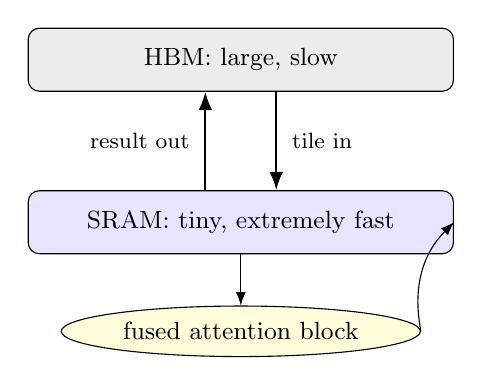
\begin{tikzpicture}[node distance=1.0cm,every node/.style={font=\small}]
  \tikzstyle{mem}=[rectangle,draw,rounded corners,minimum width=5.4cm,minimum height=0.8cm]
  \node[mem,fill=gray!15] (hbm) {HBM: large, slow};
  \node[mem,fill=blue!10,below=1.25cm of hbm] (sram) {SRAM: tiny, extremely fast};
  \node[draw,ellipse,fill=yellow!15,below=0.65cm of sram,minimum width=3.5cm] (loop) {fused attention block};
  \draw[-Latex,thick] ([xshift=0.45cm]hbm.south) --
      node[right,font=\footnotesize,align=left,xshift=2pt] {tile in} ([xshift=0.45cm]sram.north);
  \draw[-Latex,thick] ([xshift=-0.45cm]sram.north) --
      node[left,font=\footnotesize,align=right,xshift=-2pt] {result out} ([xshift=-0.45cm]hbm.south);
  \draw[-Latex] (sram) -- (loop);
  \draw[-Latex] (loop.east) to[bend left=28] (sram.east);
\end{tikzpicture}
\end{center}


The obstacle to block-wise computation is softmax, whose denominator is a sum over an \emph{entire} row:
\begin{equation}
\mathrm{softmax}(x_i) = \frac{e^{x_i}}{\sum_j e^{x_j}}.
\end{equation}
FlashAttention resolves this via the \emph{online softmax}: each tile updates running maxima and exponent sums, rescaling prior partial outputs as necessary. The algebraic identity
\begin{equation}
\ell^{(\text{new})} = e^{m^{(\text{old})} - m^{(\text{new})}} \ell^{(\text{old})} + \sum_{i \in \text{tile}} e^{x_i - m^{(\text{new})}}
\end{equation}
suffices to compute numerically stable softmax incrementally, producing exact results while never touching HBM between tiles.

\begin{remark}[There is no free lunch]
The backward pass must recompute the attention matrix, since it was never stored. The additional FLOPs are modest compared to the savings in memory traffic, and the trade is almost always worthwhile.
\end{remark}

% =====================================================================
\section{Elementwise Operations and the Fusion Hierarchy}
\label{sec:fusion}

Modern transformers interleave memory-bound elementwise operations --- RMSNorm, rotary embeddings, the SwiGLU activation $\mathrm{Sigmoid}(x) \cdot x \cdot y$, residual additions --- with heavy matrix multiplications. Each unfused operation round-trips through HBM; fused kernels collapse a chain of such operations into a single read and a single write. The toolkits for accomplishing this form a hierarchy of decreasing abstraction and increasing control:

\begin{center}
\begin{tabular}{p{3.2cm}p{11cm}}
\toprule
\textbf{Tool} & \textbf{Character} \\
\midrule
\texttt{torch.compile} & Automatic fusion of elementwise chains into Triton kernels; can orchestrate more ambitious patterns including blocked matmul fusion (as in FSDP). The correct first resort. \\
Triton                 & Python-like DSL for writing tiled, SM-level kernels; excellent middle ground and the native target of \texttt{torch.compile}. \\
CuTe                   & NVIDIA's primitives for sophisticated memory layouts; steep learning curve, indispensable for exotic tile shapes. \\
CUDA C++               & The bare metal. Maximum control, maximum development cost. Unnecessary for most use cases, irreplaceable for a few. \\
\bottomrule
\end{tabular}
\end{center}

For practitioners not inclined to write kernels, production-quality libraries exist: Liger Kernels (LinkedIn), Apex (memory-efficient RMSNorm), TransformerEngine (quantization-aware Transformer primitives), FlashAttention, and SonicMoE (specialized Mixture-of-Experts routing) are worth knowing by name.

% =====================================================================
\section{Communication Primitives}
\label{sec:nccl}


Communication among GPUs is governed by the NVIDIA Collective Communications Library (NCCL), which provides a well-defined set of primitives. These are not abstractions floating in a void; they are concrete, highly optimized algorithms with costs that can be modeled.

\begin{definition}[Collectives]
Let $G_0, \dots, G_{n-1}$ be GPUs each holding a local tensor.
\begin{description}[leftmargin=1.5em,itemsep=0.2em]
    \item[Broadcast] One root sends identical data to all GPUs.
    \item[Scatter] One root partitions its data and sends disjoint pieces to each GPU.
    \item[Gather] Each GPU sends its data to one root, which concatenates.
    \item[All-Gather] Each GPU sends its data to every other GPU; all end up with the concatenation $V_0 \oplus V_1 \oplus \cdots$.
    \item[Reduce-Scatter] Each GPU ends up with a different slice of the reduced result.
    \item[All-to-All] Each GPU sends distinct data to every other; a complete pairwise exchange.
\end{description}
\end{definition}

\subsection{Cost modeling}

A simple analytical model for an \texttt{all-to-all} is:

\begin{lstlisting}
def all_to_all_cost(bytes_gb, mesh_topo, mesh_dim):
    n   = mesh_topo.mesh_dim_devices[mesh_dim]
    bw  = mesh_topo.mesh_dim_bandwidth[mesh_dim]
    hops = n - 1
    latency = 6.6 + hops * mesh_topo.mesh_dim_latency[mesh_dim]
    bw_time = (bytes_gb * hops / n) / bw
    return latency + bw_time * 1e6   # microseconds
\end{lstlisting}

Equivalently,
\begin{align}
T_{\text{latency}} &= \tau_0 + (n-1)\, \tau_{\text{hop}}, \\
T_{\text{bandwidth}} &= \frac{\text{bytes} \cdot (n-1)/n}{\beta}, \\
T_{\text{total}} &= T_{\text{latency}} + T_{\text{bandwidth}},
\end{align}
where $\tau_0 \approx 6.6\us$ is a base overhead, $\tau_{\text{hop}}$ is the per-hop latency, and $\beta$ is the link bandwidth. The $(n-1)/n$ factor is nearly unity for large clusters but halves the bandwidth cost for $n=2$ --- a minor but consequential detail in small-world topologies.

\begin{remark}[The ring's weakest link]
In ring-based collectives, a single lagging node stalls the entire ring. The caravan moves at the speed of its slowest camel; aggregate bandwidth devolves to the minimum rate anywhere on the circle. Monitoring dashboards in production clusters routinely exhibit this signature, even when its root cause is opaque.
\end{remark}

% =====================================================================
\section{A Layer of Llama-7B}
\label{sec:llama}

To ground the preceding in something concrete, we compute the per-layer forward-pass budget for Llama-7B with
\[
S = 8192,\quad H = 4096,\quad I = 11008,\quad n_h \cdot d_h = 4096.
\]

\paragraph{Dense matmuls.}
\begin{equation}
T_{\text{matmul}} = \frac{S \cdot H \cdot (4 \cdot n_h d_h \cdot 2 + 3 \cdot I \cdot 2 + 3 \cdot S)}{800 \cdot 10^{12}} \approx 5.1\ms.
\end{equation}

\paragraph{Memory-bound glue (two RMSNorms, two residual additions, SwiGLU).}
\begin{equation}
T_{\text{mem}} = \frac{S \cdot H \cdot 2 \cdot (2 \cdot 2 + 2 \cdot 3) + S \cdot I \cdot 2 \cdot 3}{2.4 \cdot 10^{12}} \approx 0.5\ms.
\end{equation}

\paragraph{FSDP all-gather to reconstitute the sharded layer ($\approx 400\MB$).}
\begin{equation}
T_{\text{AG}} = \frac{(H \cdot n_h d_h \cdot 4 + H \cdot I \cdot 3) \cdot 2}{400 \cdot 10^{9}} \approx 1.34\ms.
\end{equation}

The hierarchy of costs is informative: matmuls ($5.1\ms$) dominate, communication ($1.34\ms$) is the secondary concern, and elementwise overhead ($0.5\ms$) is almost free. The design target is always the same: ensure communication is completely hidden behind computation.

% =====================================================================
\section{Sharding the Gargantuan: FSDP, Activation Checkpointing, Tensor Parallelism}
\label{sec:sharding}

\subsection{The activation problem}

Consider a 7B model on 1024 GPUs: roughly $26\GB$ of memory per device. For a 70B model, the demand balloons to $\sim 128\GB$, of which $\sim 120\GB$ is \emph{activations} retained for the backward pass. No amount of weight sharding alone resolves this; it is the activation ledger that explodes.

\subsection{Activation checkpointing}

\begin{remark}[The satellite analogy]
A large instrument bound for orbit is disassembled to fit the fairing and reassembled on-station. The ``waste'' of disassembly is the price of having it in space at all.
\end{remark}

Activation checkpointing is the same trade. One stores activations only at residual-connection boundaries; during the backward pass, intermediate activations are \emph{recomputed} layer-locally before gradients are propagated and discarded again. The method converts a memory cost into an extra compute cost, and the ratio is usually overwhelmingly favorable. Partial recomputation refines this further: one stores only the outputs of cheap operations and recomputes expensive intermediates on demand, so that linear-layer weight-gradient kernels can be fused with the recomputation itself.

\subsection{Tensor parallelism}

Where activation checkpointing recomputes activations, tensor parallelism ships activations \emph{to} the weights. The quintessential example is the MLP block:

\begin{center}
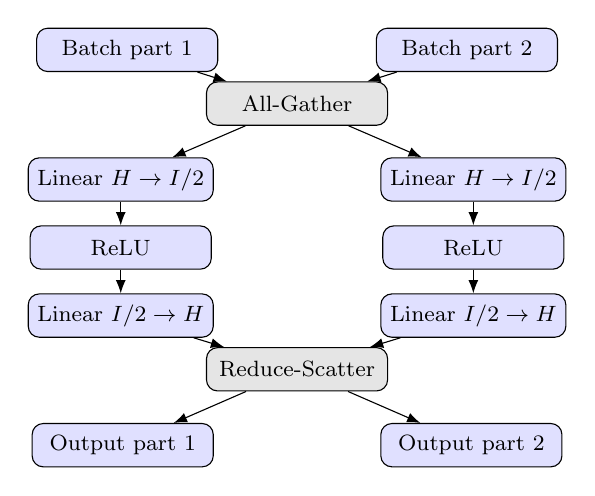
\begin{tikzpicture}[node distance=0.7cm, every node/.style={font=\footnotesize}]
  \tikzstyle{b}=[draw,rounded corners,minimum width=2.3cm,minimum height=0.55cm,fill=blue!12]
  \tikzstyle{c}=[draw,rounded corners,minimum width=2.3cm,minimum height=0.55cm,fill=gray!20]
  
  \node[b] (in1) {Batch part 1};
  \node[b,right=2cm of in1] (in2) {Batch part 2};
  \node[c,below=0.4cm of $(in1)!0.5!(in2)$] (ag) {All-Gather};
  \node[b,below left=0.4cm and -0.1cm of ag] (l1a) {Linear $H \to I/2$};
  \node[b,below right=0.4cm and -0.1cm of ag] (l1b) {Linear $H \to I/2$};
  \node[b,below=0.3cm of l1a] (r1) {ReLU};
  \node[b,below=0.3cm of l1b] (r2) {ReLU};
  \node[b,below=0.3cm of r1] (l2a) {Linear $I/2 \to H$};
  \node[b,below=0.3cm of r2] (l2b) {Linear $I/2 \to H$};
  \node[c,below=0.4cm of $(l2a)!0.5!(l2b)$] (rs) {Reduce-Scatter};
  \node[b,below left=0.4cm and -0.1cm of rs] (o1) {Output part 1};
  \node[b,below right=0.4cm and -0.1cm of rs] (o2) {Output part 2};
  
  \draw[-Latex] (in1) -- (ag); \draw[-Latex] (in2) -- (ag);
  \draw[-Latex] (ag) -- (l1a); \draw[-Latex] (ag) -- (l1b);
  \draw[-Latex] (l1a) -- (r1); \draw[-Latex] (l1b) -- (r2);
  \draw[-Latex] (r1) -- (l2a); \draw[-Latex] (r2) -- (l2b);
  \draw[-Latex] (l2a) -- (rs); \draw[-Latex] (l2b) -- (rs);
  \draw[-Latex] (rs) -- (o1); \draw[-Latex] (rs) -- (o2);
\end{tikzpicture}
\end{center}

The weight matrix is split column-wise for the first linear, row-wise for the second. An all-gather precedes, a reduce-scatter follows, and the composition is \emph{mathematically identical} to the monolithic block. Attention admits a parallel split along heads, which is structurally equivalent. For a 70B layer at TP=8, typical per-layer costs are roughly $10\ms$ of matmul against $4\ms$ of collective and $0.5\ms$ of elementwise work --- communication is present but manageable on NVLink.

\subsection{Asynchronous tensor parallelism}

Synchronous TP stalls computation during the all-gather. Asynchronous TP interleaves them: as small tiles of input arrive, the first linear immediately consumes them; the downstream linear is paired with a reduce-scatter operating in parallel. The gain is substantial, particularly when the per-tile computations are themselves small enough that kernel-launch overhead dominates.

% =====================================================================
\section{Case Studies at Scale}
\label{sec:cases}

\subsection{Qwen 3 (235B)}
\begin{center}
\begin{tabular}{ll}
\toprule
Per-layer size (BF16)              & $5\GB$ \\
Optimal forward ($S = 8k$)         & $5\ms$ \\
Optimal FSDP communication         & $12.5\ms$ \\
\bottomrule
\end{tabular}
\end{center}
Communication outpaces compute by $2.5 \times$. Two levers restore balance: double the local batch to $16k$ (computation doubles; communication stays constant) and halve the communicated bytes by shipping weights in FP8 rather than BF16. The \texttt{reduce-scatter}, which aggregates gradients across thousands of GPUs, remains in FP32 to avoid accumulation drift.

\subsection{DeepSeek v3 (671B)}
\begin{center}
\begin{tabular}{ll}
\toprule
Per-layer size (BF16)              & $21\GB$ \\
Optimal forward ($S = 8k$)         & $10\ms$ \\
Optimal FSDP communication         & $57\ms$ \\
\bottomrule
\end{tabular}
\end{center}
Here communication exceeds compute by nearly $6\times$, and even holding two layers of weights and gradients simultaneously overflows HBM. No single lever suffices; one needs pipelining, expert parallelism, aggressive quantization, and careful scheduling in concert.

% =====================================================================
\section{Mixture of Experts}
\label{sec:moe}


A Mixture-of-Experts (MoE) layer replaces a single dense MLP with a pool of experts $\{E_1, \ldots, E_E\}$ and a router. For each token, the router selects the top-$k$ experts; the token's output is the weighted sum of their outputs. A common configuration is $E = 256$ experts with $k = 8$ active per token: the model has enormous capacity, but the FLOPs per token remain those of a $k$-expert dense equivalent.

\begin{center}
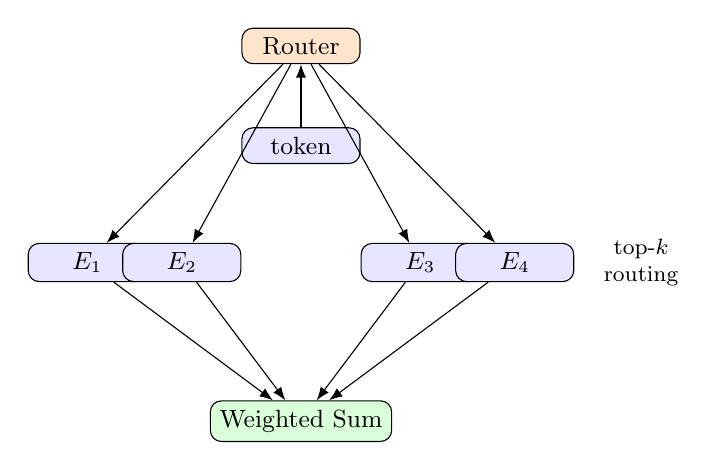
\begin{tikzpicture}[node distance=0.9cm, every node/.style={font=\small}]
  \tikzstyle{b}=[draw,rounded corners,fill=blue!10,minimum width=1.5cm]
  \node[b] (tok) {token};
  \node[b,above=0.8cm of tok,fill=orange!20] (rt) {Router};
  \node[b,below left=1cm and 1.2cm of tok] (e1) {$E_1$};
  \node[b,below left=1cm and 0cm of tok] (e2) {$E_2$};
  \node[b,below right=1cm and 0cm of tok] (e3) {$E_3$};
  \node[b,below right=1cm and 1.2cm of tok] (e4) {$E_4$};
  \node[b,below=3cm of tok,fill=green!15] (ws) {Weighted Sum};
  \draw[-Latex] (tok) -- (rt);
  \draw[-Latex] (rt) -- (e1); \draw[-Latex] (rt) -- (e2);
  \draw[-Latex] (rt) -- (e3); \draw[-Latex] (rt) -- (e4);
  \draw[-Latex] (e1) -- (ws); \draw[-Latex] (e2) -- (ws);
  \draw[-Latex] (e3) -- (ws); \draw[-Latex] (e4) -- (ws);
  \node[font=\footnotesize,align=center,right=0.25cm of e4] {top-$k$\\ routing};
\end{tikzpicture}
\end{center}

Efficient MoE execution requires a \emph{permutation} that groups tokens by assigned expert, yielding contiguous streams suitable for GroupedGEMM. Tokens routed to multiple experts are replicated. Load imbalance is managed by token-dropping with a small $k$-overhead (perhaps a $15\%$ increase in $k$) to reduce loss.

\subsection{Tensor vs.\ expert parallelism}

\begin{description}[leftmargin=1.5em,itemsep=0.3em]
    \item[Tensor Parallelism (TP)] splits each expert's weight matrices across GPUs. Communication: all-gather + permute + reduce-scatter. Appropriate on fast (NVLink) fabrics.
    \item[Expert Parallelism (EP)] assigns entire experts to distinct GPUs. Communication: dispatch tokens to the right GPU, run expert locally, combine. The memory footprint is lower because the weights are not duplicated, but routing introduces irregular all-to-all traffic.
\end{description}

\begin{example}[GroupedGEMM at $S=8192$, $E=256$, $k=8$, $H=7168$, $I=2048$]
For TP=8:
\begin{align}
T_{\text{comp}} &= \frac{(S \cdot TP) \cdot k \cdot H \cdot (I/TP) \cdot 2}{800 \cdot 10^{12}} \approx 2.5\ms, \\
T_{\text{mem}}  &= \frac{(S \cdot TP \cdot k \cdot H + E \cdot H \cdot I / TP) \cdot 2}{2.4 \cdot 10^{12}} \approx 3.5\ms.
\end{align}
Memory-bound by a slim margin.
For EP=8 the memory term drops dramatically to $0.78\ms$ (each GPU touches only $E/k$ experts locally). The all-gather/reduce-scatter overhead on TP=8 is roughly $2.2\ms$ per side; set against a $10\ms$ forward pass, a $4.4\ms$ total communication cost is substantial but, in principle, overlappable with the compute of a second batch.
\end{example}

% =====================================================================
\section{Pipeline Parallelism}
\label{sec:pipeline}

When the model is too deep to shard any other way, one cuts it \emph{transversally}: stages of $N$ consecutive layers are placed on distinct devices, and micro-batches flow through the stages as water through locks.



The fundamental inefficiency is the \emph{pipeline bubble}: at startup, only one stage has work; at teardown, only one stage remains. Schedules such as 1F1B interleave forward and backward passes of distinct micro-batches to reduce activation memory pressure. Refinements --- ZeroBubble (ZB-H1, ZB-H2), DualPipeV --- separate the backward pass into ``gradient of inputs'' and ``gradient of weights'' sub-stages, exploiting the fact that the weight-gradient computation can be deferred to the optimizer step, further compacting the schedule.

\subsection{Inter-node communication}

For residual tensors (roughly $2$ bytes per token) transmitted across a single NIC port,
\begin{equation}
T_{\text{residual}} = \frac{S \cdot H \cdot 2}{50 \cdot 10^{9}} \approx 2\ms.
\end{equation}
This is small compared to per-stage compute of tens of milliseconds, which makes pipeline parallelism attractive even across slow inter-node links. Backward passes, which compute gradients for both outputs and weights, nominally take twice the forward time --- a fact that schedules like ZeroBubble exploit by decoupling the two computations.

% =====================================================================
\section{Context Parallelism and Long Sequences}
\label{sec:ctx}


At sequence lengths of $10^5$ tokens and beyond, even FlashAttention's memory savings cease to suffice: a single query sequence of $8k$ joined to a KV history of $64k$ on a batch of $64$ is already beyond a single H100. Two families of solutions have emerged.

\subsection{Ring attention}

Ring attention pipelines KV blocks around a ring of GPUs. Each GPU holds a shard of $Q$ and receives, in turn, every shard of $K,V$ from its neighbors, computing attention incrementally in the FlashAttention manner. To avoid the imbalance between first and last shards (the latter accumulates the full softmax history), a symmetric allocation is adopted: each GPU holds the $k$-th and the $(N-k+1)$-th fragments, so all GPUs share the boundary load equally.

\subsection{Ulysses}

The Ulysses strategy is structurally simpler. It performs an \texttt{all-to-all} exchange so that, after the transpose, each GPU holds a subset of \emph{heads} for the \emph{full} sequence. Attention is then computed locally (typically with FlashAttention), and a second \texttt{all-to-all} restores the original layout. The method trades ring-style streaming communication for two bursts of dense all-to-all --- often a favorable trade when bandwidth is abundant and implementation simplicity is at a premium.

\begin{center}
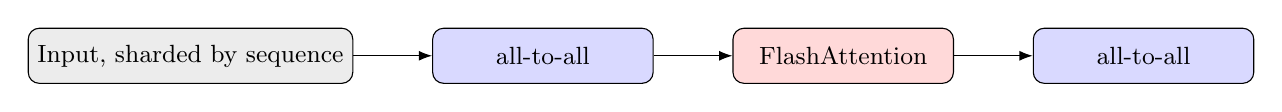
\begin{tikzpicture}[node distance=1cm, every node/.style={font=\small}]
  \tikzstyle{b}=[draw,rounded corners,minimum width=2.8cm,minimum height=0.7cm]
  \node[b,fill=gray!15] (in) {Input, sharded by sequence};
  \node[b,fill=blue!15,right=of in] (a1) {all-to-all};
  \node[b,fill=red!15,right=of a1] (fa) {FlashAttention};
  \node[b,fill=blue!15,right=of fa] (a2) {all-to-all};
  \draw[-Latex] (in) -- (a1);
  \draw[-Latex] (a1) -- (fa);
  \draw[-Latex] (fa) -- (a2);
\end{tikzpicture}
\end{center}

% =====================================================================
\section{Automated Parallelization}
\label{sec:auto}

Choosing the right combination of data parallelism, tensor parallelism, pipeline parallelism, context parallelism, and expert parallelism is, in principle, a discrete optimization problem whose objective function is the estimated iteration time derived from the cost models of \S\ref{sec:nccl} and \S\ref{sec:llama}. Recent tooling (e.g., PyTorch's \texttt{AutoParallel}) attempts to automate this: given a compiled module, the system decomposes it, analyzes data dependencies, and proposes a sharding plan.

The direction of travel is clear, if not yet fully traveled: the practitioner specifies the model and the hardware; the compiler searches the joint space of parallelism strategies and emits a performant plan. The three classical flavors --- data, task, and pipeline parallelism --- compose hierarchically, and what were once expert choices will increasingly become compiler choices. The contextual and retentive constraints of correctness --- causal masks, KV-cache consistency, numerical stability across shards --- remain the province of the human.

% =====================================================================

\end{document}
